\documentclass[a4paper, twoside, utf8]{ctexart}
\usepackage[fontset=Fandol]{ctex}
\usepackage{anyfontsize}
\usepackage{subcaption}
\usepackage{adjustbox}
\usepackage{algorithm}
\usepackage{longtable}
\usepackage{abstract}
\usepackage{amsfonts}
\usepackage{appendix}
\usepackage{booktabs}
\usepackage{enumitem}
\usepackage{fancyhdr}
\usepackage{geometry}
\usepackage{graphicx}
\usepackage{tabularx}
\usepackage{listings}
\usepackage{amsmath}
\usepackage{caption}
\usepackage{lipsum}
\usepackage{minted}
\usepackage{xcolor}
\usepackage{array}
\usepackage{url}

\geometry{a4paper,left=31mm,right=31mm,top=25mm,bottom=25mm}
\setlength{\parindent}{2em}
\ctexset{section = {format = \raggedright\large\bfseries}}
\let\oldsection\section
\renewcommand{\abstracttextfont}{\normalsize}

\pagestyle{fancy}
\fancyhf{}
\fancyhead[CO,CE]{议程管理系统 \ Agenda}
\fancyhead[LE]{编译器构造实验}
\fancyhead[RO]{Lab02测试文档}
\fancyhead[RE,LO]{}
\fancyfoot[CO]{\thepage}
\fancyfoot[CE]{\thepage}
\fancyfoot[LE,RE]{}
\fancyfoot[LO,RO]{}

\title{\songti \bfseries 议程管理系统 \ 测试文档}
\author{\fangsong 傅祉珏 \ \ 21307210}
\date{\fangsong 中山大学计算机学院\ 广东广州\ 510006}

\begin{document}
	
	\begin{titlepage}
		\centering
		\rule{\textwidth}{1pt}
		\vspace{0.02\textheight}
		
		{\LARGE \kaishu 编译器构造实验 \quad Lab02测试文档}
		
		\vspace{0.02\textheight}
		
		{\Huge \songti \bfseries 议程管理系统}
		
        \vspace{0.025\textheight}
        \rule{0.83\textwidth}{0.4pt}
        \vspace{0.05\textheight} 
        
        \begin{figure}[htbp]
            \centering
            
\includegraphics[width=8cm, height=8cm]{./figure/计院院徽.jpg}
        \end{figure}

        \vspace{0.05\textheight} 
        {\Large 课程编号:\textsc{DCS292}}

        \vspace{0.025\textheight} 
        {\Large 学生姓名:\textsc{傅祉珏}}

        \vspace{0.025\textheight} 
        {\Large 学生学号:\textsc{21307210}}

        \vspace{0.025\textheight} 
        {\Large 指导老师:\textsc{李文军\ 教授}}
 
        \vspace{0.025\textheight} 
        {\Large 项目截止日期:\textsc{2025年4月10日}}

        \vspace{0.05\textheight} 
        \vfill

        {\large \today}
        \vspace{0.1\textheight}
        \rule{\textwidth}{1pt}
    \end{titlepage}
	
    \pagenumbering{Roman}
    \setcounter{page}{1}
    \renewcommand{\abstractname}{\Large \textbf{摘要}}
    \addcontentsline{toc}{section}{摘要}
    \begin{abstract}
        本测试文档围绕编译器构造课程 Lab02 实验项目“议程管理系统”的设计与实现,系统性地开展了一系列功能性与性能性测试。该系统作为一次面向对象工程开发实践,以命令行交互为核心,支持用户注册、登录、创建会议、查询会议及删除会议等会议生命周期管理操作,旨在帮助学生在实践中深化对封装、继承、多态等面向对象编程思想的理解,掌握高内聚低耦合的软件架构设计方法。

        本文档重点对系统所采用的四层架构模型(UI、BLL、DML、DAL)进行分层测试与验证,确保各模块在功能实现、接口协同与异常处理方面具备高度稳定性与一致性。测试内容涵盖业务逻辑验证、数据管理完整性、IO 性能评估等多个维度,采用单元测试、交互测试与性能测试等多种手段进行综合评估。测试结果表明,系统各模块功能完备,响应迅速,具备良好的健壮性和可维护性,能够满足日常使用及高负载场景下的运行需求。文档中亦指出系统当前在会议数据持久化策略方面存在的性能瓶颈,并提出针对性优化建议,体现了测试过程中的工程化思维和问题反馈机制。
    
        本测试工作的全面性与系统性不仅有效提升了实验项目的整体质量,也为后续更复杂的编译器实验项目打下了坚实的基础。
        
        \vspace{1em}
        \noindent{\textbf{\heiti 关键词:}议程管理系统、编译器实验、分层架构、单元测试、IO性能优化。}
    \end{abstract}
    \newpage

    \addcontentsline{toc}{section}{目录}
    \begingroup
    \setcounter{tocdepth}{2}
    \renewcommand{\section}{
        \renewcommand{\raggedright}{}
        \ctexset{section/format = \centering\Large\bfseries}
        \oldsection
    }
    \tableofcontents
    \endgroup
    \newpage

    \pagenumbering{arabic}
    \setcounter{page}{1}
	
	\maketitle

    \section{项目概述}

    \subsection{项目背景与目标}

    本项目作为编译器构造课程中的 Lab02 实验任务,承接 Lab01 中对 Java 编程语言基本语法和面向对象思想的初步掌握,旨在通过构建议程管理系统这一完整工程项目,进一步提升在面向对象编程、系统设计与程序结构组织方面的综合实践能力。实验重点不仅在于实现一个功能完备的会议管理工具,更在于通过项目开发过程深化对封装、继承、多态等核心特性的理解与应用,同时引入异常处理机制、模块化架构思想与常用设计模式,在真实工程环境中掌握构建高内聚、低耦合系统的关键方法。

    系统整体以命令行交互作为操作入口,支持用户注册、登录、创建会议、查询会议、删除会议等一系列会议生命周期管理功能。用户在系统中可通过输入标准命令实现各类操作,系统将通过解析命令、执行业务逻辑、维护数据状态并进行持久化等步骤,完成对功能流程的完整支持。通过本次实验,不仅能够锻炼在复杂系统中进行逻辑抽象与功能拆分的能力,还能积累实际开发中对系统可靠性、扩展性及可维护性等方面的工程经验,为后续更高复杂度的编译原理实验奠定坚实的理论与技术基础。

    \subsection{系统架构设计}

    议程管理系统采用经典的四层架构模型进行分层设计,包括用户界面层(UI)、业务逻辑层(BLL)、数据管理层(DML)以及数据持久层(DAL),通过结构清晰、职责分明的体系架构实现各功能模块的协同运行与解耦管理。其中,用户界面层通过命令行方式与用户交互,负责解析输入命令、分发指令及反馈执行结果;业务逻辑层负责对用户对象与会议对象的行为进行抽象与封装,处理系统中各类业务逻辑判断;数据管理层作为业务层与持久层之间的桥梁,负责维护内存中实体对象的状态,并协调数据更新与同步操作;数据持久层则利用本地文件系统实现数据的存储、读取与恢复,确保数据的持久化与系统重启后的状态一致性。

    各层之间通过标准化的接口进行调用,从而实现高内聚低耦合的模块交互关系。例如,UI 层接收到用户指令后将请求传递至 BLL 层,经过逻辑判断与数据处理后再由 DML 层协调 DAL 层进行数据存储,整个过程清晰有序,符合单一职责原则。该架构不仅利于功能模块的独立测试与验证,也为后期系统的升级扩展提供了良好的基础,体现出良好的工程实践与软件设计理念。

    \begin{figure}
        \centering
        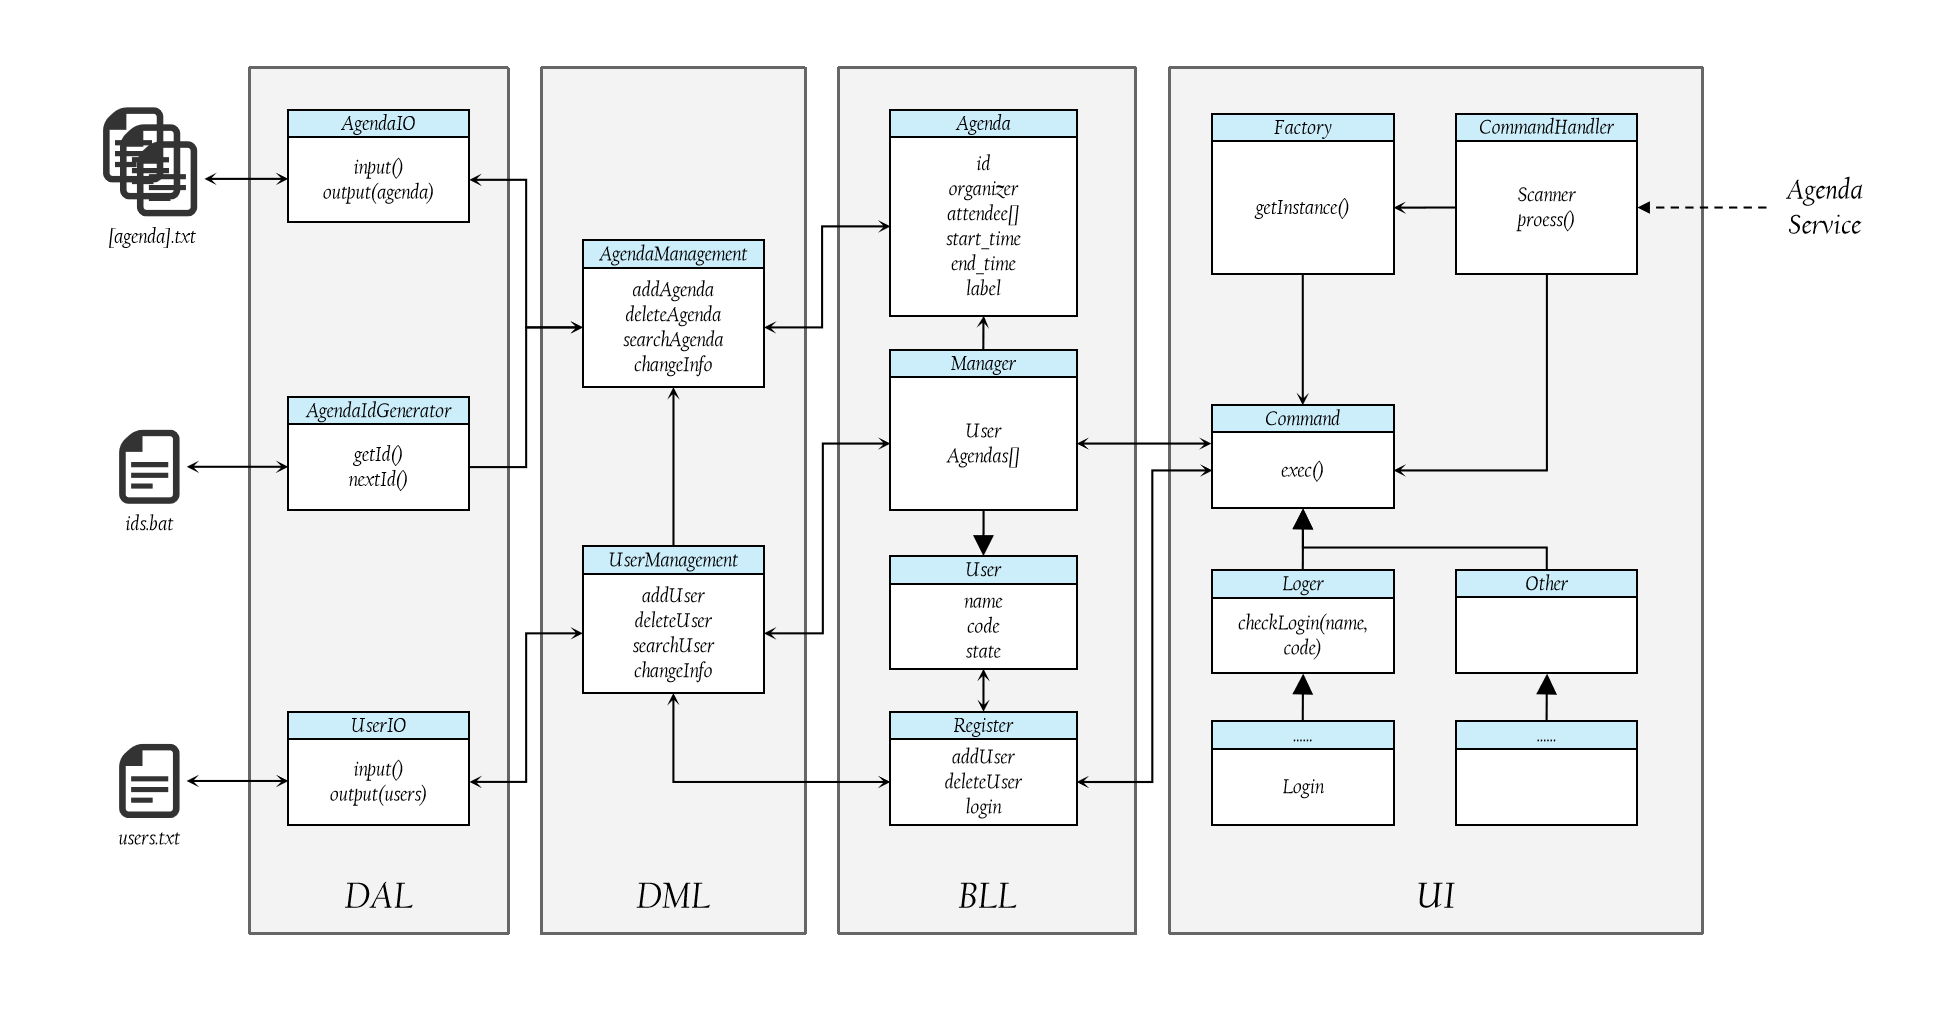
\includegraphics[width=.9\linewidth]{figure/structure.png}
        \caption{系统架构设计图}
    \end{figure}

    \section{测试方案简介}

    \subsection{测试目标与范围}

    本测试方案旨在全面验证议程管理系统在四层架构模型下的正确性、稳定性及协同工作能力。测试目标聚焦于用户界面层(UI)、业务逻辑层(BLL)、数据管理层(DML)以及数据持久层(DAL)各自是否能独立完成各自的核心职责,并在层与层之间的接口交互中保持逻辑正确性与数据一致性。系统各层职责明确,若能分别通过功能验证测试,则整个系统在接口调用和流程控制上的协调性也可得到间接验证。因此,测试将覆盖从模块功能实现到模块间调用的全过程,不仅关注模块功能的“是否能用”,更强调系统在实际运行场景下的“是否可靠”、“是否高效”。此外,测试还将评估系统在异常输入、边界条件等复杂情况下的行为表现,确保最终系统的健壮性和用户体验质量。

    \subsection{测试方法设计}

    为满足测试目标并覆盖系统各层次功能与性能要求,本次测试采用混合测试方法策略,结合单元测试、性能测试与交互测试三种手段进行全方位验证。对于业务逻辑层、数据管理层以及数据持久层,主要通过 JUnit 测试框架设计和编写系统单元测试用例,重点测试各类接口方法的功能完整性、异常处理能力以及边界输入条件下的表现。同时,为提升系统性能评估的全面性,将引入时间记录机制对高频调用方法进行性能测试,分析其在不同数据规模下的响应速度和资源消耗。

    针对用户界面层,因其依赖命令行输入和实时交互特性,难以使用传统单元测试进行模拟验证,因此采用用户实测与对比测试相结合的方式。通过模拟真实用户操作流程,手动输入系统支持的各类命令,观察命令解析、指令执行及结果反馈过程是否符合预期,与现有的命令行软件进行对比检查命令行界面及指令集设计的合理性,并重点测试系统对非法输入、异常命令的处理反应。此外,还将组织小规模用户测试,通过收集使用反馈,进一步评估系统在使用便利性、出错提示、交互友好性等方面的表现。该设计保证了测试既有程序级验证,也涵盖了实际用户行为视角,确保系统在投入使用前已具备较高的稳定性与易用性。

    \section{业务逻辑测试}

    \subsection{测试目标}

    本次测试的主要目标是验证业务逻辑层中核心抽象类——用户类与会议议程类的功能完整性与逻辑准确性。作为系统功能的核心承载者,用户类与会议类不仅承接着系统的数据结构与行为逻辑的设计理念,更直接关联到系统是否能够正确完成用户注册、认证、会议创建与管理等核心业务流程。因此,该层的测试旨在确保这两个类在完成其抽象职责的同时,能够支持系统预期中的功能需求,具备良好的可扩展性与健壮性,为上层交互与下层数据管理提供稳定支撑。

    \subsection{测试用例设计}

    测试用例围绕用户类与会议议程类的主要功能展开,分别从对象的创建、信息的修改与功能性操作三个维度进行验证。在对象创建方面,用户类支持“用户名+密码”的标准构造方式,以及拷贝构造方式的深复制机制,测试中验证了两种方式均能正确返回逻辑等价但内存独立的用户对象;会议类则支持带编号和不带编号的构造方式,测试确保不同构造方式下对象的核心属性初始化一致,功能等效。

    信息更改测试方面,用户类支持用户名与密码的变更操作,测试用例在连续更改与边界条件下验证了数据的有效更新。会议类则实现了组织者和会议标签的修改功能,测试中确保变更操作在数据层能够实时反映,且不影响其他属性的完整性。会议时间修改功能暂未在当前版本中实现,后续将补充相应测试。

    在功能性测试方面,用户类支持用户名比对与密码验证逻辑,该功能是系统用户认证模块的关键基础。测试中使用多个用户名与密码组合验证匹配准确性,并确保错误输入时返回正确结果。会议类的功能性操作包括添加参会者与删除参会者,测试用例覆盖了单个、多名、重复添加与边界删除等多种情况,确保会议类中参会者列表的完整性与一致性不被破坏。

    \subsection{测试结果与问题记录}

    通过 JUnit 框架对用户类与会议类进行单元测试,所有功能测试用例均顺利通过,系统行为与预期一致。在性能方面,用户类在执行全部三项测试内容(创建、更改信息、验证操作)时平均耗时为 86.1ms,会议类平均耗时为 130.1ms,均处于合理范围内,体现了良好的运行效率。

    测试过程中暂未发现功能性Bug,类方法间依赖关系明确,边界情况处理恰当,未出现异常终止或逻辑错误。少数在重复添加参会者的测试中,需进一步明确系统业务规则(如是否允许重复用户),该问题已在测试记录中标注,建议后续在业务逻辑设计中加以规范与处理。总体而言,业务逻辑层实现达到了功能正确、性能可控、结构清晰的预期目标,具备良好的系统支撑能力。

    \begin{figure}[htbp]
        \centering
        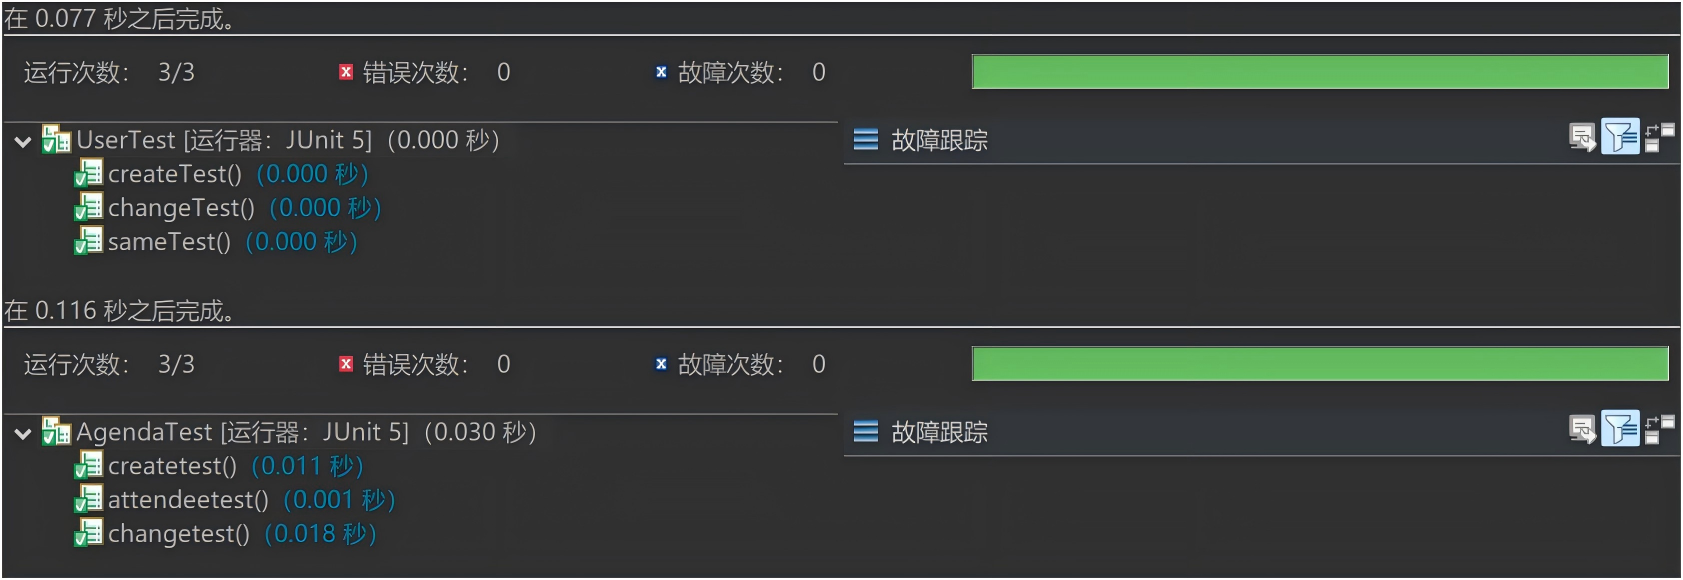
\includegraphics[width=.9\linewidth]{figure/GeneralTest.png}
        \caption{业务逻辑测试结果}
    \end{figure}

    \section{数据管理测试}

    \subsection{测试目标}

    数据管理层作为连接业务逻辑与持久化存储的中间桥梁,其主要职责是完成系统运行期间对用户与会议数据的增、删、查、改操作。在本次测试中,主要目标是验证用户管理类与会议管理类在功能实现上是否能够覆盖基本数据操作的完整性,是否能在正常与异常情况下稳定运行,并对常见异常情形进行识别和有效处理,确保系统在数据管理过程中的一致性与健壮性。

    \subsection{测试用例设计}

    用户数据管理部分测试主要围绕用户的添加、删除与查询展开,测试过程中适当穿插用户信息修改操作,以检验系统在多路径数据调用中的稳定性。测试首先模拟向系统中添加两个拥有相同用户名的用户,此时系统应能捕捉到用户名唯一性约束冲突并抛出相应错误码,避免错误数据写入。随后更改其中一名用户的用户名并重新尝试添加操作,测试系统是否能在修改后正确接纳该用户。对于查询操作,测试既包括查询已存在的用户名,亦包括尝试查询一个不存在的用户名,系统应分别返回有效用户对象与空对象,以供后续流程判断使用。删除操作则在删除前后分别执行查询操作,确保用户被成功移除并在系统中不可再检索到。

    会议数据管理部分的测试更为复杂,不仅需完成基本的数据操作验证,还需联合用户数据进行交叉验证。首先,在添加会议的测试中,系统应能准确识别会议时间段的冲突,若尝试添加两个时间上存在重叠的会议,则系统应拒绝后者的添加请求,并返回失败信息。若两个会议时间段无冲突,则应顺利完成添加。会议的查询功能较为多样,测试分别验证了三类典型查询路径:查询某一用户的全部会议、查询特定会议ID对应的会议记录,以及按时间段查询某一用户的会议列表,系统应分别返回与查询条件相匹配的会议集合。会议删除功能的测试则类似于用户管理部分,通过删除前后查询的方式验证会议记录是否被成功移除,并确保系统状态同步更新。

    测试结束后,为避免测试数据干扰后续操作或造成持久化数据污染,所有测试用例执行完成后均包含清理流程,对测试期间新增的用户与会议数据进行彻底清除,确保测试过程对系统运行环境无残留影响。

    \subsection{测试结果与问题记录}

    采用 JUnit 框架对用户管理类与会议管理类分别进行了系统性单元测试,测试用例覆盖所有主要功能路径与典型边界条件,测试结果表明系统行为稳定,功能表现与设计预期一致。在性能方面,用户管理类执行全部测试用例的平均耗时为 123.6ms,而会议管理类完成对应测试的平均耗时为 190.9ms,单项操作平均耗时均控制在 100ms 左右,显示出良好的响应速度与数据处理能力。

    测试过程中未发现功能性Bug,系统在处理重复数据、非法查询与冲突添加等异常情况下均能正确识别并返回标准错误响应,体现了良好的容错能力。测试结尾阶段所执行的清理流程也有效恢复了系统至测试前状态,保证了系统数据的独立性与测试环境的整洁性。整体而言,数据管理模块通过了本轮功能与稳定性验证,具备支撑上层业务逻辑与底层持久化的能力。

    \begin{figure}[htbp]
        \centering
        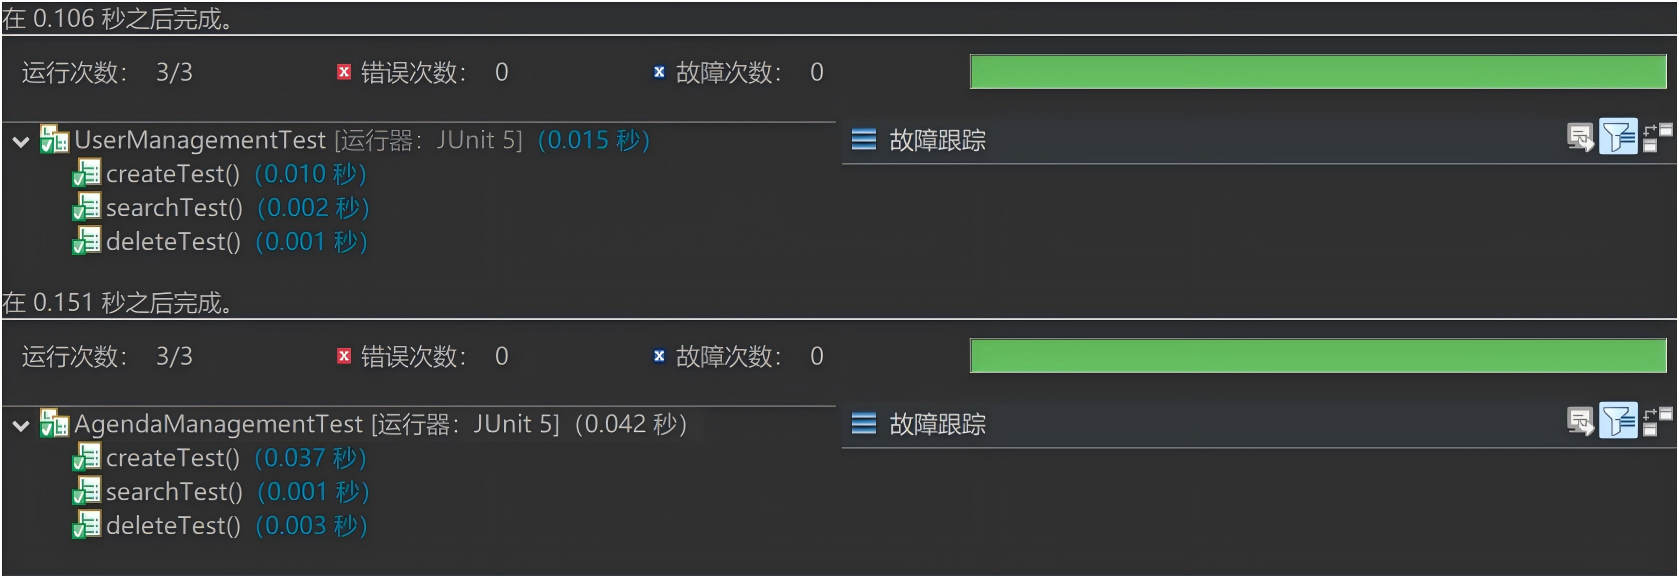
\includegraphics[width=.9\linewidth]{figure/ManagementTest.png}
        \caption{数据管理测试结果}
    \end{figure}

    \section{IO性能测试}

    \subsection{测试目标}

    在议程管理系统中,除核心的数据逻辑与管理功能外,确保系统具备良好的实时交互体验同样至关重要。若系统在数据读写过程中的响应时间较长,将直接影响用户的操作流畅性与整体使用感受。因此,IO性能的优劣成为评估系统质量的关键因素之一。尤其是在数据量较大或并发操作频繁的情况下,IO操作是否能够高效完成,直接关系到系统能否持续稳定运行。本轮IO性能测试的主要目标,是验证系统在不同数据量级下进行输入(数据读入)和输出(数据写出)操作的能力,确保在日常使用乃至高负载场景下均能保持良好的响应效率,从而为用户提供流畅、实时的操作体验。
    
    \subsection{测试用例设计}

    针对系统中的持久化操作,主要测试对象为用户类与会议议程类的数据持久化实现。二者的IO操作均可抽象为两类基本操作:数据输入,即将外部存储(如文件系统)中的内容加载至系统内存;数据输出,即将系统中更新后的内容保存至外部存储。因此测试策略将围绕这两类基本操作展开,对其在不同数据量场景下的性能表现进行评估。

    为更全面评估系统的IO处理能力,本次测试分为三个阶段:第一阶段为单例测试,用于验证在最小单位数据量下系统的读写延迟是否处于合理范围;第二阶段为批量测试,采用每类对象10个实例,检验系统在一般负载情况下的IO处理能力;第三阶段为压力测试,模拟大数据量条件下的读写操作。具体而言,用户类将在压力测试中加载和写入1000个用户数据,而会议议程类则处理100个会议记录。每组测试均在添加与删除两个操作场景下分别进行,过程中通过高精度计时记录IO操作的起止时间,作为系统IO响应性能的依据。

    \subsection{测试结果与优化建议}

    测试过程中,使用 JUnit 框架对用户类和会议议程类的IO操作进行逐项评估,测试结果显示系统整体具备良好的IO处理性能,特别是在普通和中等负载条件下,操作响应迅速,满足实时性要求。具体而言,在压力测试中,用户类在一次性添加1000条用户数据时,耗时仅为 461.1ms,而删除这部分数据耗时也控制在 374.6ms。相较而言,会议议程类在处理100条会议记录时,添加与删除的耗时分别为 1573.5ms 与 1426.7ms,明显高于用户类的IO耗时。

    通过分析可知,造成会议议程类IO耗时较长的原因主要在于当前的写入策略:在每次执行添加或删除操作时,系统会先清空原有会议记录文件,再将全部会议数据重新写入。尽管此方法能够确保数据一致性与文件状态的正确性,但在数据规模扩大后,重复写入操作显著增加了时间开销,导致整体IO性能下降。

    基于以上分析,建议在未来版本中对会议议程类的持久化策略进行优化。一种可行的优化方案是引入缓冲区机制,即在内存中维护一个数据缓冲池,先将变动内容写入缓冲区,待所有数据变更操作完成后统一进行文件写入。这种“批量刷新”的方式不仅能够减少磁盘写入的次数,也能有效避免不必要的重复清空与覆盖操作,从而大幅提升大数据量处理时的IO性能。

    本轮测试中的所有计时与性能数据均已整理归档于附录B。其中,IO测试1、批量测试1 与 压力测试1 分别对应添加数据操作下的单例测试、批量测试与压力测试;而 IO测试2、批量测试2 与 压力测试2 则对应删除数据操作下的各类测试情境,具体数值可供未来性能对比与优化参考使用。整体而言,议程管理系统当前的IO性能表现已基本满足实验目标与交互响应需求,但仍存在进一步优化的空间,特别是在会议数据的批处理与高并发场景下。

    \begin{figure}[htbp]
        \centering
        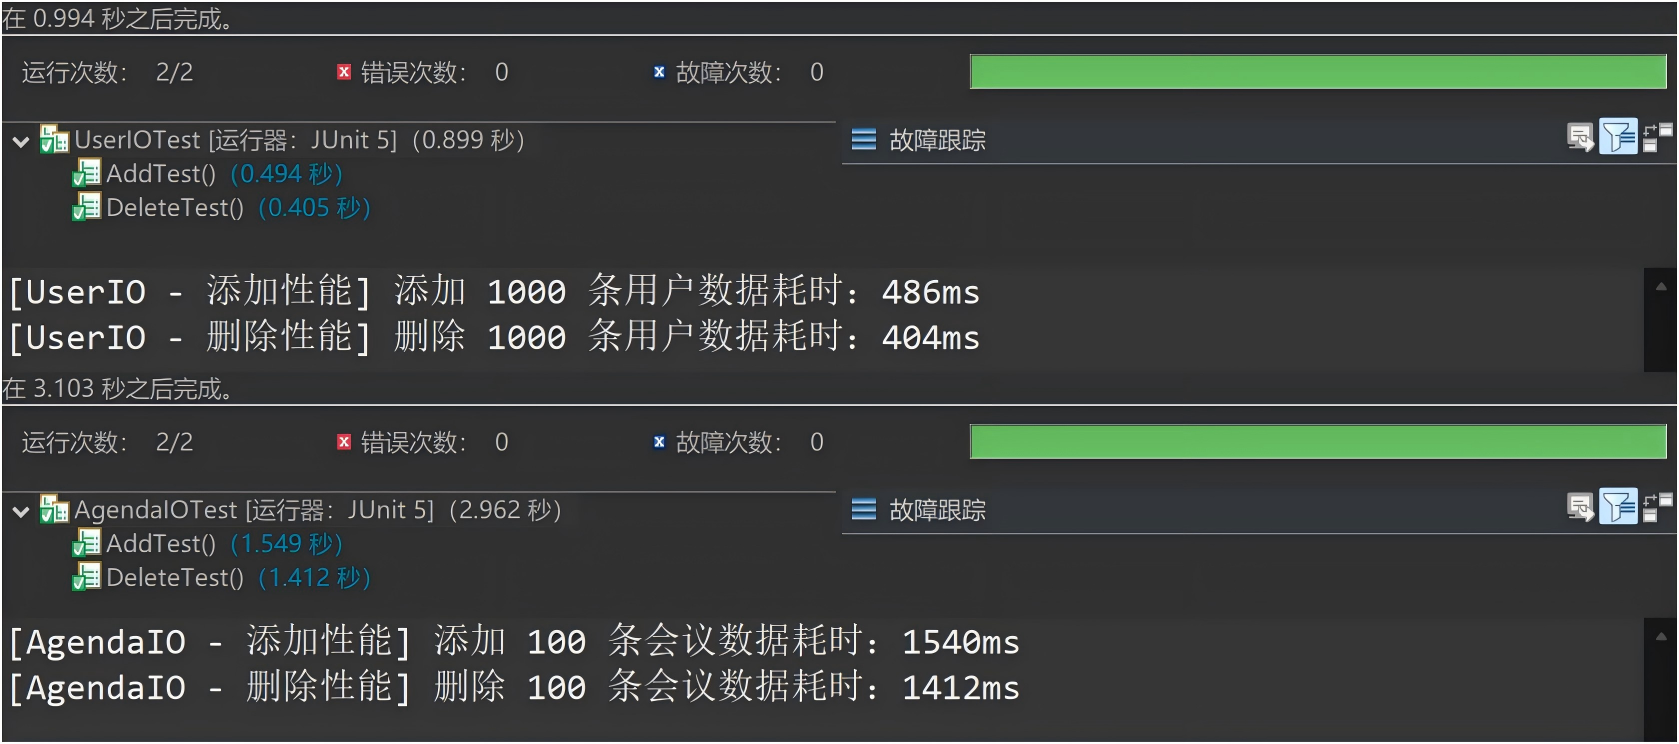
\includegraphics[width=.9\linewidth]{figure/IOTest.png}
        \caption{IO性能测试结果}
    \end{figure}

    \section{用户交互测试}

    \subsection{测试目标}

    用户交互测试的核心目标在于验证系统命令行交互界面的可用性与稳定性,尤其是在面对不同类型的输入命令及异常行为时的处理能力。由于UI界面及异常行为具有一定的灵活性和主观性,难以通过 JUnit 等自动化单元测试工具进行全面覆盖,因此采用用户实测的方式进行。本次测试旨在通过模拟实际用户操作过程,考察系统命令行交互是否直观、指令执行是否准确,以及系统在应对错误输入时是否能够提供清晰的反馈。同时,为了提升评估的客观性与对比性,选取了市面上主流的命令行工具(如 Miniconda)作为参照对象,对界面交互的合理性与用户体验进行综合分析。

    \subsection{测试结果与用户体验反馈}

    在界面友好性方面,通过与 Miniconda 命令行工具进行对比测试,可以看出本系统所设计的命令行交互界面结构清晰,指令分布合理,帮助信息完整,能够有效引导用户执行所需操作。用户能够较为容易地掌握命令使用方式,并快速完成注册、登录、创建会议等操作,整体交互流程符合一般用户的使用习惯。

    \begin{figure}[htbp]
        \begin{minipage}{.5\textwidth}
            \centering
            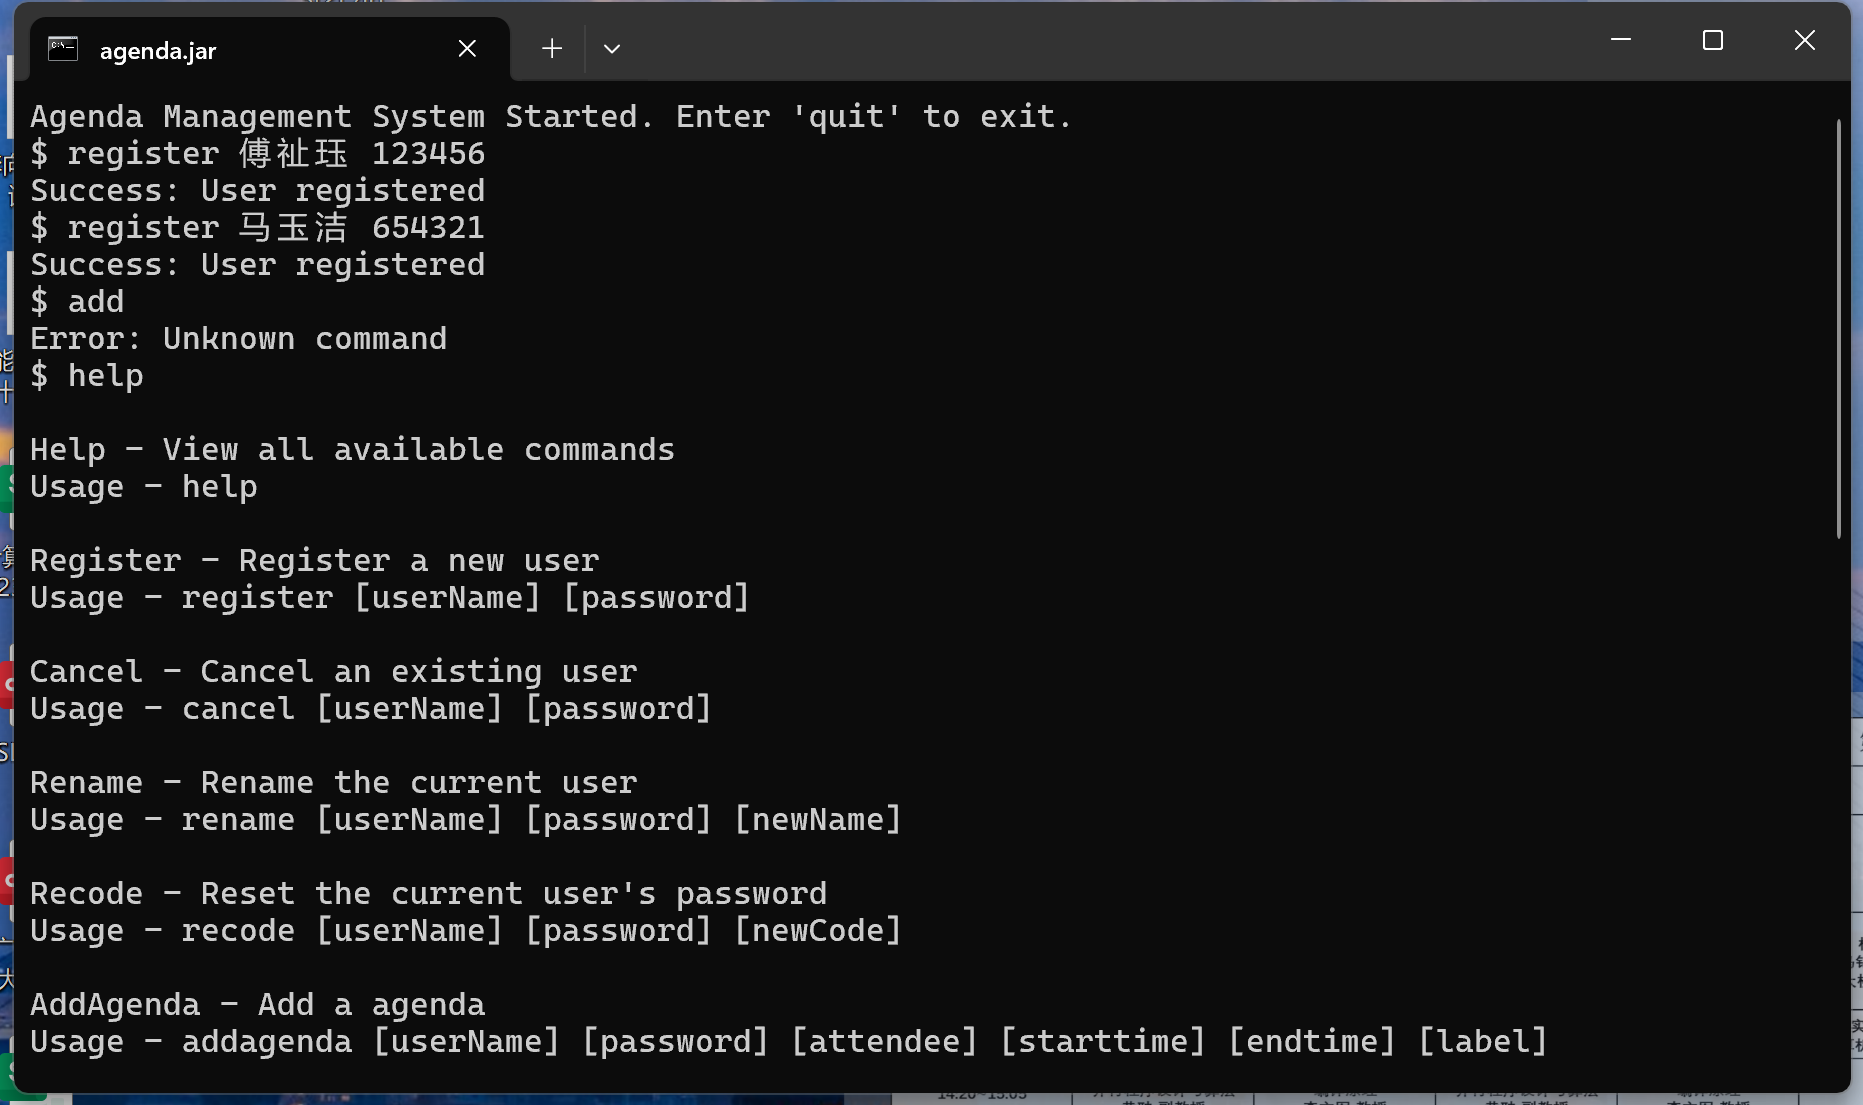
\includegraphics[height=.15\textheight]{figure/ui.png}
            \caption{用户交互测试示意}
        \end{minipage}
        \begin{minipage}{.45\textwidth}
            \centering
            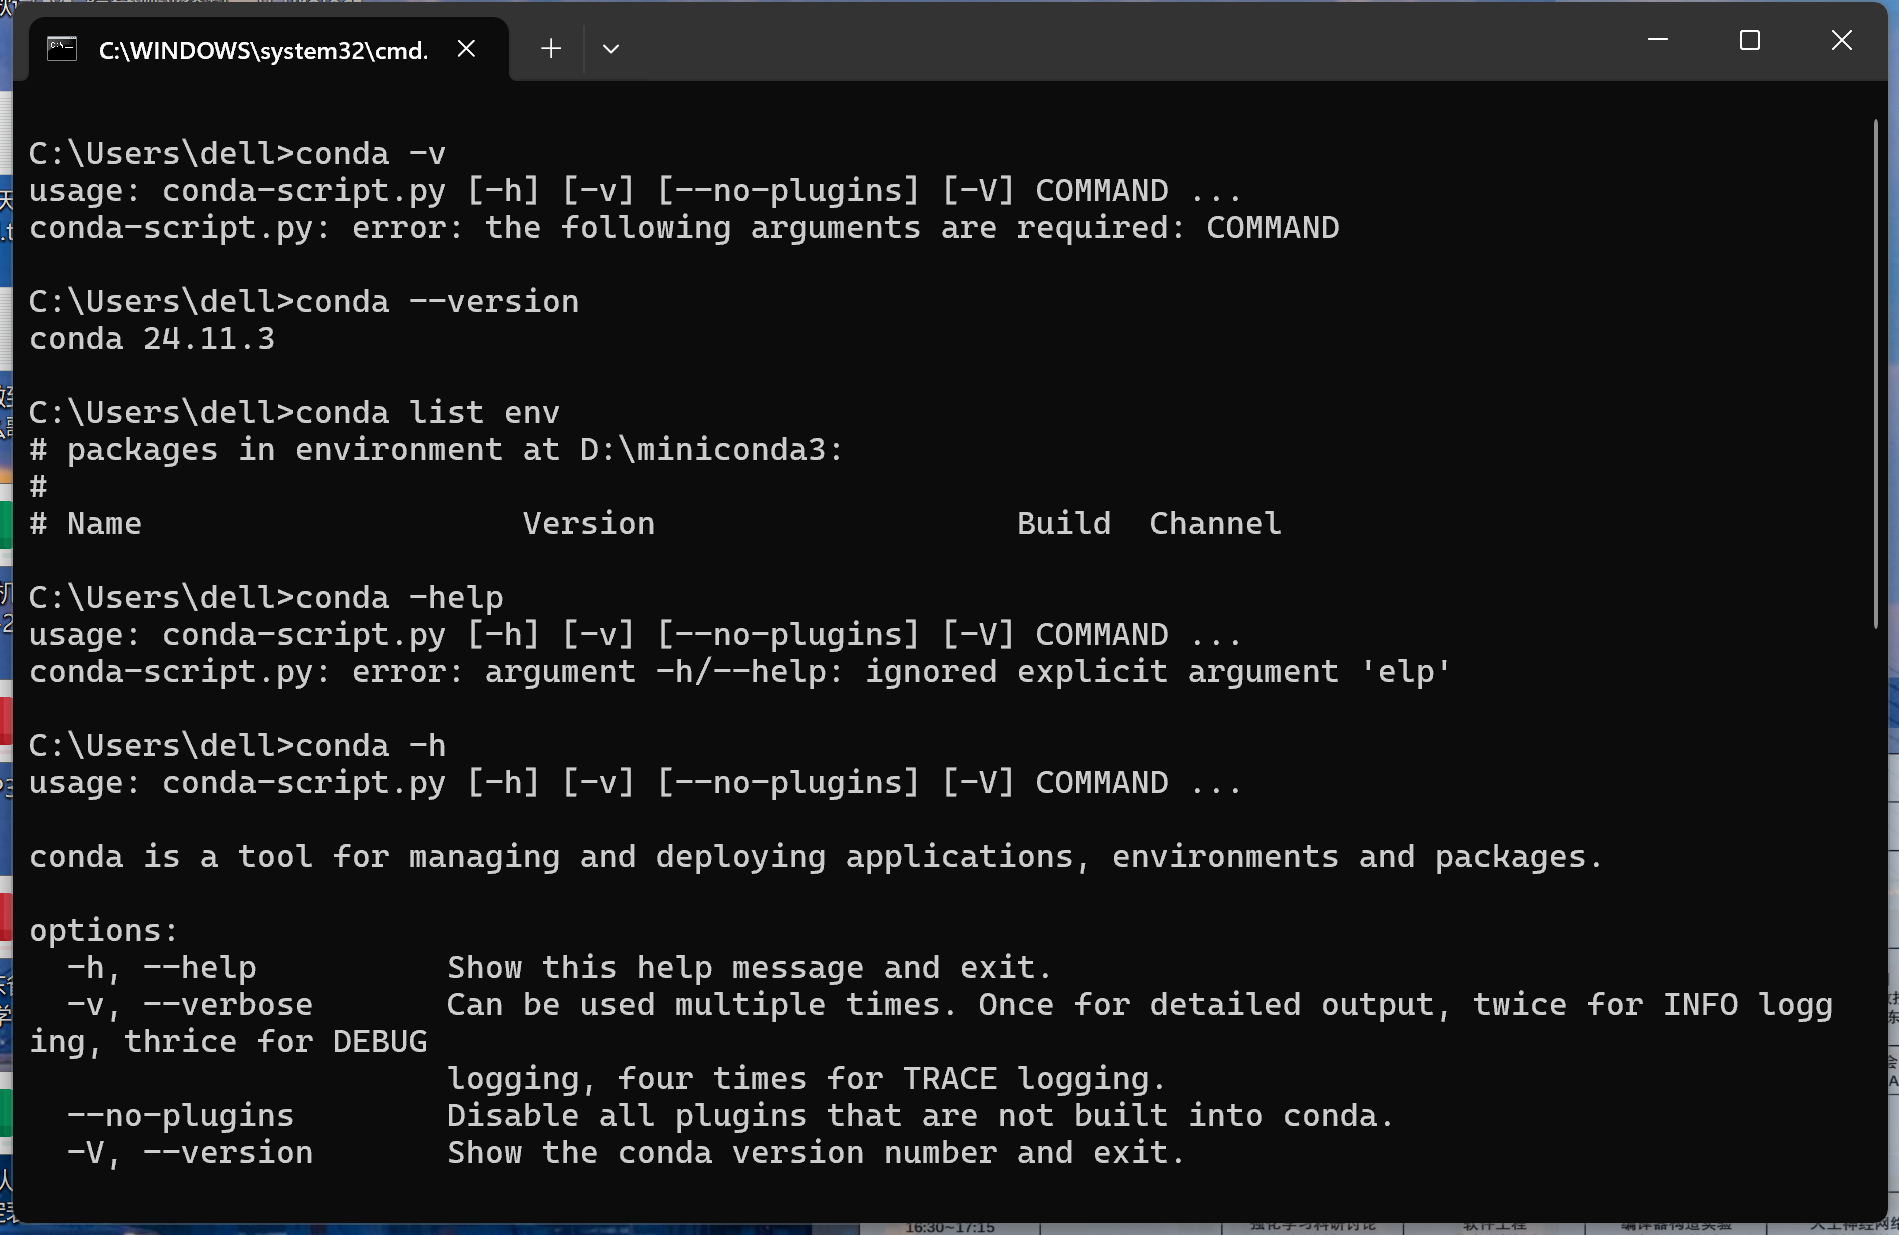
\includegraphics[height=.15\textheight]{figure/conda.png}
            \caption{miniconda 界面}
        \end{minipage}
    \end{figure}

    在异常行为测试中,测试人员故意输入错误命令、缺失参数、重复操作等无效指令,以检验系统的异常处理能力。测试结果表明,系统具备良好的错误识别与提示机制,能够对无效命令、参数错误或权限不足等问题及时作出响应,并通过明确的提示信息引导用户修正输入,有效提升了使用体验与系统容错性。

    最终用户实测阶段,共有多名测试用户参与体验,覆盖不同使用场景与操作习惯。根据测试反馈统计,系统整体用户满意度超过 90\%,其中多数用户认可系统的交互清晰度与使用便利性。不过,也有部分用户反馈在使用中文进行命令输入与数据持久化操作时,可能出现字符集编码问题,如命令无法识别或输出乱码等现象。此问题主要由字符集不兼容导致,尤其在命令行输出与文件存储过程中更为明显。因此建议在实际使用过程中尽量以英文作为输入输出语言,避免频繁使用中文,以确保系统交互过程的稳定性与可读性。未来版本将考虑引入统一编码方案或多语言支持机制,进一步提升系统的国际化与兼容性。
	
    \addcontentsline{toc}{section}{参考文献}
    \begin{thebibliography}{99}
        \bibitem{ref1} 沐言科技\ 李兴华.\ Java编程\ 从入门到实践[M].\ 第1版.\ 安徽:中国水利水电出版社,\ 2021.
        \bibitem{ref2} 毛新军,\ 董威.\ 软件工程——理论与实践[M].\ 第1版.\ 北京:高等教育出版社,\ 2024.
    \end{thebibliography}
	
	\newpage
	\appendix
	\centerline{\Large{\textbf{附录}}}

    \section{测试用例列表}

    \begin{itemize}[itemsep=2pt, topsep=0pt, parsep=0pt]
        \item \verb|UserTest| \quad 用户测试类
        \item \verb|AgendaTest| \quad 会议测试类
        \item \verb|UserManagementTest| \quad 用户管理测试类
        \item \verb|AgendaManagementTest| \quad 会议管理测试类
        \item \verb|TestDataGenerator| \quad 测试用例生成类
        \item \verb|UserIOTest| \quad 用户IO测试类
        \item \verb|AgendaIOTest| \quad 会议日程IO测试类
    \end{itemize}

    \section{性能测试数据表}

    \begin{center}
        \setlength{\LTcapwidth}{\textwidth}
        
        \small
        
        \begin{longtable}{
            >{\centering\arraybackslash}m{.08\textwidth}
            | >{\centering\arraybackslash}m{.08\textwidth}
            | >{\centering\arraybackslash}m{.08\textwidth}
            | >{\centering\arraybackslash}m{.08\textwidth}
            | >{\centering\arraybackslash}m{.08\textwidth}
            | >{\centering\arraybackslash}m{.08\textwidth}
            | >{\centering\arraybackslash}m{.08\textwidth}
            | >{\centering\arraybackslash}m{.08\textwidth}
            | >{\centering\arraybackslash}m{.08\textwidth}
        }
            
            \toprule
            单位\ ms & \multicolumn{2}{c|}{核心测试} & \multicolumn{2}{c|}{管理测试} & \multicolumn{2}{c|}{IO测试1} & \multicolumn{2}{c}{批量测试1} \\
            测试号 & User & Agenda & User & Agenda & User & Agenda & User & Agenda \\
            \midrule
            \endfirsthead
            
            \multicolumn{9}{l}{\footnotesize 续表} \\
            \toprule
            单位\ ms & \multicolumn{2}{c|}{核心测试} & \multicolumn{2}{c|}{管理测试} & \multicolumn{2}{c|}{IO测试1} & \multicolumn{2}{c}{批量测试1} \\
            测试号 & User & Agenda & User & Agenda & User & Agenda & User & Agenda \\
            \midrule
            \endhead
            
            \midrule
            \multicolumn{9}{r}{\footnotesize 接下页}
            \endfoot
            
            \bottomrule
            \endlastfoot

            1 & 92 & 185 & 130 & 199 & 1 & 7 & 4 & 43 \\
            2 & 78 & 140 & 139 & 205 & 0 & 9 & 4 & 36 \\
            3 & 77 & 144 & 101 & 191 & 0 & 8 & 5 & 39 \\
            4 & 79 & 151 & 94 & 178 & 1 & 14 & 5 & 48 \\ 
            5 & 89 & 110 & 131 & 201 & 1 & 7 & 4 & 48 \\ 
            6 & 86 & 113 & 127 & 193 & 1 & 7 & 4 & 41 \\
            7 & 81 & 114 & 123 & 192 & 1 & 8 & 4 & 51 \\ 
            8 & 97 & 114 & 135 & 193 & 1 & 8 & 4 & 35 \\
            9 & 90 & 115 & 130 & 188 & 1 & 12 & 4 & 45 \\
            10 & 92 & 115 & 126 & 169 & 2 & 7 & 5 & 56 \\
            \midrule
            AVE & 86.1 & 130.1 & 123.6 & 190.9 & 0.9 & 8.7 & 4.3 & 44.2 \\

            
        \end{longtable}
        \vspace{-3em}
    \end{center}

    \begin{center}
        \setlength{\LTcapwidth}{\textwidth}
        
        \small
        
        \begin{longtable}{
            >{\centering\arraybackslash}m{.08\textwidth}
            | >{\centering\arraybackslash}m{.08\textwidth}
            | >{\centering\arraybackslash}m{.08\textwidth}
            | >{\centering\arraybackslash}m{.08\textwidth}
            | >{\centering\arraybackslash}m{.08\textwidth}
            | >{\centering\arraybackslash}m{.08\textwidth}
            | >{\centering\arraybackslash}m{.08\textwidth}
            | >{\centering\arraybackslash}m{.08\textwidth}
            | >{\centering\arraybackslash}m{.08\textwidth}
        }
            
            \toprule
            单位\ ms & \multicolumn{2}{c|}{压力测试1} & \multicolumn{2}{c|}{IO测试2} & \multicolumn{2}{c|}{批量测试2} & \multicolumn{2}{c}{压力测试2} \\
            测试号 & User & Agenda & User & Agenda & User & Agenda & User & Agenda \\
            \midrule
            \endfirsthead
            
            \multicolumn{9}{l}{\footnotesize 续表} \\
            \toprule
            单位\ ms & \multicolumn{2}{c|}{压力测试1} & \multicolumn{2}{c|}{IO测试2} & \multicolumn{2}{c|}{批量测试2} & \multicolumn{2}{c}{压力测试2} \\
            测试号 & User & Agenda & User & Agenda & User & Agenda & User & Agenda \\
            \midrule
            \endhead
            
            \midrule
            \multicolumn{9}{r}{\footnotesize 接下页}
            \endfoot
            
            \bottomrule
            \endlastfoot

            1 & 600 & 1570 & 0 & 0 & 3 & 24 & 357 & 1427 \\
            2 & 461 & 1555 & 0 & 1 & 3 & 22 & 372 & 1390 \\
            3 & 440 & 1540 & 1 & 1 & 4 & 24 & 365 & 1418 \\
            4 & 437 & 1557 & 1 & 0 & 4 & 22 & 369 & 1497 \\
            5 & 446 & 1569 & 1 & 0 & 4 & 22 & 368 & 1376 \\
            6 & 440 & 1604 & 0 & 1 & 3 & 24 & 370 & 1415 \\
            7 & 431 & 1579 & 1 & 1 & 4 & 22 & 403 & 1406 \\
            8 & 453 & 1557 & 0 & 0 & 4 & 23 & 389 & 1449 \\
            9 & 446 & 1639 & 2 & 1 & 4 & 25 & 394 & 1459 \\
            10 & 457 & 1565 & 1 & 1 & 4 & 25 & 359 & 1430 \\
            \midrule
            AVE & 461.1 & 1573.5 & 0.7 & 0.6 & 3.7 & 23.3 & 374.6 & 1426.7 \\
            
        \end{longtable}
        \vspace{-3em}
    \end{center}

    \section{用户反馈信息}

    为进一步完善系统功能与提升用户体验,我们在测试阶段收集了部分用户的反馈意见。以下列出其中两位用户的典型反馈内容,诚挚感谢所有参与测试的用户,正是这些宝贵的建议与评价,将有助于议程管理系统在未来实现更加完善与智能的升级优化。

    \subsection{Ma D 反馈信息}

    在对该议程管理系统进行全面评测后,我认为该系统整体设计较为合理,功能划分明确,覆盖了用户注册、密码重置、议程的增删改查及与会者管理等关键操作,并且还提供了批量命令执行和开发者信息查询功能,极大地方便了用户在命令行下对会议的管理。系统对命令语法的说明详细,易于理解使用,对常见错误的容错机制以及退出命令的设置也让操作更为流畅。虽然系统的核心功能已经具备,但在细节处理和界面友好性方面还有进一步优化空间,比如对输入格式的严谨性检验、错误信息的提示以及批量操作时的日志记录等方面可以进一步完善。从安全性角度出发,用户权限管理和会议信息隐私保护等方面也建议加入更多细粒度的设置与校验。总体而言,这套基于命令行的议程管理系统结构清晰,操作便捷,适用于中小规模会议管理,能够满足基本的日常使用需求,因此我给予该系统 95.3/100 的评分。

    \subsection{Huang J R 反馈信息}

    这款议程管理系统绝对称得上是会议管理的高效助手,整体表现相当出色,我愿意给它 90 分的高分!虽然目前仅提供命令行界面,但界面设计简洁直观,操作逻辑清晰,无论是创建日程、设置提醒还是管理参会人员,功能都非常一目了然,用起来特别顺手。系统的本地运行方式虽然暂未支持多端联动,但也正因如此,它运行稳定、响应迅速,特别适合个人用户或在单机环境下集中处理日常会议安排。冲突检测功能尤其实用,能自动提醒时间重叠的会议安排,帮我避免了不少日程冲突的尴尬。此外,议程管理中的细节也做得非常到位,比如参会人员列表管理、会议备注、提醒机制等,覆盖了会议组织的关键需求。要说改进空间的话,我希望未来版本可以提供图形化界面,提高可视化体验;同时也非常期待它支持多端同步功能,这样无论是在公司电脑还是出差用的笔记本上,都能方便地查看和管理会议日程。
	
\end{document}
